\chapter{Numbers 21}


\begin{figure}
  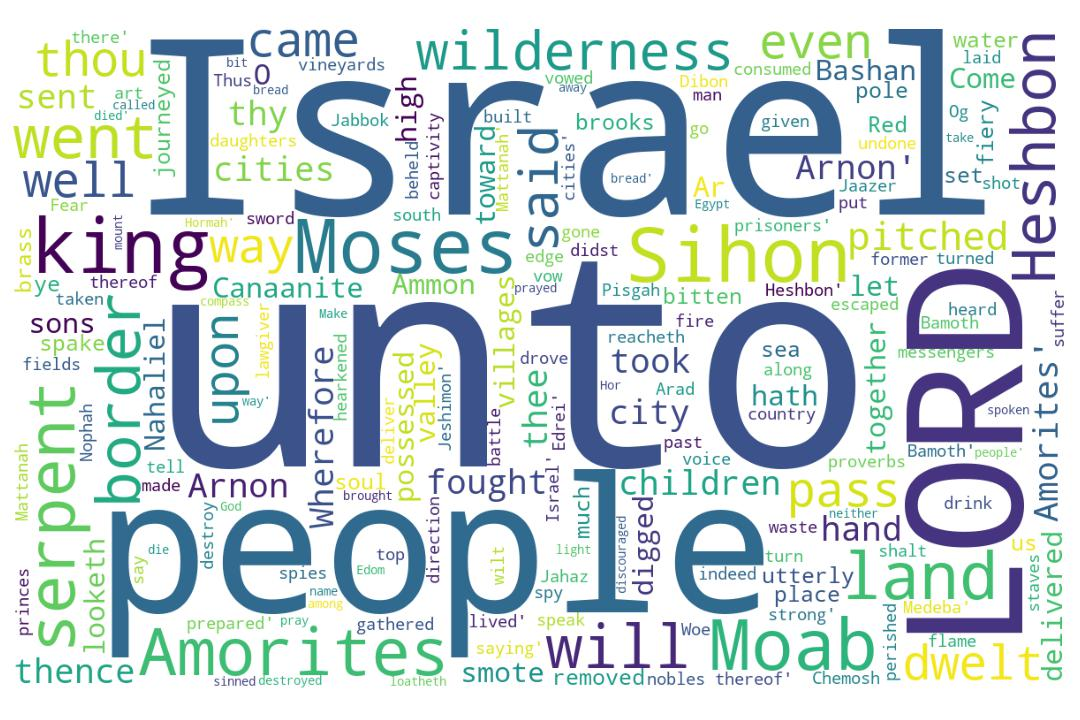
\includegraphics[width=\linewidth]{04OT-Numbers/Numbers21-WordCloud.jpg}
  \caption{Numbers 21 Word Cloud}
  \label{fig:Numbers 21 word Cloud}
\end{figure}


\marginpar{\scriptsize \centering \fcolorbox{bone}{lime}{\textbf{SIN, SERPENTS \& SWORDS}}\\ (Numbers 21)
\begin{compactenum}[I.][8]
     \item  The \textbf{Sin} of Discouragement \index[scripture]{Numbers!Num 21:04}   (Numbers 21:4)
    \item  \textbf{Serpents}  \index[scripture]{Numbers!Num 21:06}   (Numbers 21:6)
    \item  \textbf{Supplication}  \index[scripture]{Numbers!Num 21:07}   (Numbers 21:7)
    \item  The \textbf{Symbol}  \index[scripture]{Numbers!Num 21:09}   (Numbers 21:9)
    \item  A \textbf{Song}  \index[scripture]{Numbers!Num 21:17}   (Numbers 21:17)
    \item  The \textbf{Sword}  \index[scripture]{Numbers!Num 21:24}   (Numbers 21:24)
\end{compactenum}}




\footnote{\textcolor[rgb]{0.00,0.25,0.00}{\hyperlink{NumbersTOC}{Return to end of Table of Contents.}}}\footnote{\href{https://audiobible.com/bible/numbers_21.html}{\textcolor[cmyk]{0.99998,1,0,0}{Numbers 21 Audio}}}\textcolor[cmyk]{0.99998,1,0,0}{And \emph{when} king Arad the Canaanite, which dwelt in the south, heard tell that Israel came by the way of the spies; then he fought against Israel, and took \emph{some} of them prisoners.}
[2] \textcolor[cmyk]{0.99998,1,0,0}{And Israel vowed a vow unto the LORD, and said, If thou wilt indeed deliver this people into my hand, then I will utterly destroy their cities.}
[3] \textcolor[cmyk]{0.99998,1,0,0}{And the LORD hearkened to the voice of Israel, and delivered up the Canaanites; and they utterly destroyed them and their cities: and he called the name of the place Hormah.}\\
\\
\P \textcolor[cmyk]{0.99998,1,0,0}{And they journeyed from mount Hor by the way of the Red sea, to compass the land of Edom: and the soul of the people was much discouraged because of the way.}
[5] \textcolor[cmyk]{0.99998,1,0,0}{And the people spake against God, and against Moses, Wherefore have ye brought us up out of Egypt to die in the wilderness? for \emph{there} \emph{is} no bread, neither \emph{is} \emph{there} \emph{any} water; and our soul loatheth this light bread.}
[6] \textcolor[cmyk]{0.99998,1,0,0}{And the LORD sent fiery serpents among the people, and they bit the people; and much people of Israel died.}\\
\\
\P \textcolor[cmyk]{0.99998,1,0,0}{Therefore the people came to Moses, and said, We have sinned, for we have spoken against the LORD, and against thee; pray unto the LORD, that he take away the serpents from us. And Moses prayed for the people.}
[8] \textcolor[cmyk]{0.99998,1,0,0}{And the LORD said unto Moses, Make thee a fiery serpent, and set it upon a pole: and it shall come to pass, that every one that is bitten, when he looketh upon it, shall live.}
[9] \textcolor[cmyk]{0.99998,1,0,0}{And Moses made a serpent of brass, and put it upon a pole, and it came to pass, that if a serpent had bitten any man, when he beheld the serpent of brass, he lived.}\\
\\
\P \textcolor[cmyk]{0.99998,1,0,0}{And the children of Israel set forward, and pitched in Oboth.}
[11] \textcolor[cmyk]{0.99998,1,0,0}{And they journeyed from Oboth, and pitched at Ije-abarim, in the wilderness which \emph{is} before Moab, toward the sunrising.}
[12] \textcolor[cmyk]{0.99998,1,0,0}{From thence they removed, and pitched in the valley of Zared.}
[13] \textcolor[cmyk]{0.99998,1,0,0}{From thence they removed, and pitched on the other side of Arnon, which \emph{is} in the wilderness that cometh out of the coasts of the Amorites: for Arnon \emph{is} the border of Moab, between Moab and the Amorites.}
[14] \textcolor[cmyk]{0.99998,1,0,0}{Wherefore it is said in the book of the wars of the LORD, What he did in the Red sea, and in the brooks of Arnon,}
[15] \textcolor[cmyk]{0.99998,1,0,0}{And at the stream of the brooks that goeth down to the dwelling of Ar, and lieth upon the border of Moab.}
[16] \textcolor[cmyk]{0.99998,1,0,0}{And from thence \emph{they} \emph{went} to Beer: that \emph{is} the well whereof the LORD spake unto Moses, Gather the people together, and I will give them water.}
[17] \textcolor[cmyk]{0.99998,1,0,0}{Then Israel sang this song, Spring up, O well; sing ye unto it:}
[18] \textcolor[cmyk]{0.99998,1,0,0}{The princes digged the well, the nobles of the people digged it, by \emph{the} \emph{direction} \emph{of} the lawgiver, with their staves. And from the wilderness \emph{they} \emph{went} to Mattanah:}
[19] \textcolor[cmyk]{0.99998,1,0,0}{And from Mattanah to Nahaliel: and from Nahaliel to Bamoth:}
[20] \textcolor[cmyk]{0.99998,1,0,0}{And from Bamoth \emph{in} the valley, that \emph{is} in the country of Moab, to the top of Pisgah, which looketh toward Jeshimon.}\\
\\
\P \textcolor[cmyk]{0.99998,1,0,0}{And Israel sent messengers unto Sihon king of the Amorites, saying,}
[22] \textcolor[cmyk]{0.99998,1,0,0}{Let me pass through thy land: we will not turn into the fields, or into the vineyards; we will not drink \emph{of} the waters of the well: \emph{but} we will go along by the king's \emph{high} way, until we be past thy borders.}
[23] \textcolor[cmyk]{0.99998,1,0,0}{And Sihon would not suffer Israel to pass through \fcolorbox{bone}{bone}{his} border: but Sihon gathered all \fcolorbox{bone}{bone}{his} people together, and went out against Israel into the wilderness: and he came to Jahaz, and fought against Israel.}
[24] \textcolor[cmyk]{0.99998,1,0,0}{And Israel smote him with the edge of the sword, and possessed \fcolorbox{bone}{bone}{his} land from Arnon unto Jabbok, even unto the children of Ammon: for the border of the children of Ammon \emph{was} strong.}
[25] \textcolor[cmyk]{0.99998,1,0,0}{And Israel took all these cities: and Israel dwelt in all the cities of the Amorites, in Heshbon, and in all the villages thereof.}
[26] \textcolor[cmyk]{0.99998,1,0,0}{For Heshbon \emph{was} the city of Sihon the king of the Amorites, who had fought against the former king of Moab, and taken all \fcolorbox{bone}{bone}{his} land out of \fcolorbox{bone}{bone}{his} hand, even unto Arnon.}
[27] \textcolor[cmyk]{0.99998,1,0,0}{Wherefore they that speak in proverbs say, Come into Heshbon, let the city of Sihon be built and prepared:}
[28] \textcolor[cmyk]{0.99998,1,0,0}{For there is a fire gone out of Heshbon, a flame from the city of Sihon: it hath consumed Ar of Moab, \emph{and} the lords of the high places of Arnon.}
[29] \textcolor[cmyk]{0.99998,1,0,0}{Woe to thee, Moab! thou art undone, O people of Chemosh: he hath given \fcolorbox{bone}{bone}{his} sons that escaped, and \fcolorbox{bone}{bone}{his} daughters, into captivity unto Sihon king of the Amorites.}
[30] \textcolor[cmyk]{0.99998,1,0,0}{We have shot at them; Heshbon is perished even unto Dibon, and we have laid them waste even unto Nophah, which \emph{reacheth} unto Medeba.}\\
\\
\P \textcolor[cmyk]{0.99998,1,0,0}{Thus Israel dwelt in the land of the Amorites.}
[32] \textcolor[cmyk]{0.99998,1,0,0}{And Moses sent to spy out Jaazer, and they took the villages thereof, and drove out the Amorites that \emph{were} there.}
[33] \textcolor[cmyk]{0.99998,1,0,0}{And they turned and went up by the way of Bashan: and Og the king of Bashan went out against them, he, and all \fcolorbox{bone}{bone}{his} people, to the battle at Edrei.}
[34] \textcolor[cmyk]{0.99998,1,0,0}{And the LORD said unto Moses, Fear him not: for I have delivered him into thy hand, and all \fcolorbox{bone}{bone}{his} people, and \fcolorbox{bone}{bone}{his} land; and thou shalt do to him as thou didst unto Sihon king of the Amorites, which dwelt at Heshbon.}
[35] \textcolor[cmyk]{0.99998,1,0,0}{So they smote him, and \fcolorbox{bone}{bone}{his} sons, and all \fcolorbox{bone}{bone}{his} people, until there was none left him alive: and they possessed \fcolorbox{bone}{bone}{his} land.}